\chapter{\textit{FrontEnd}}
Di seguito viene illustrato la parte di \textit{FrontEnd} del progetto. Verranno illustrate le principali funzionalità sviluppate ed alcuni dettagli implementativi.

\section{\textit{Home Page}}
    \begin{figure}[H]
        \centering
        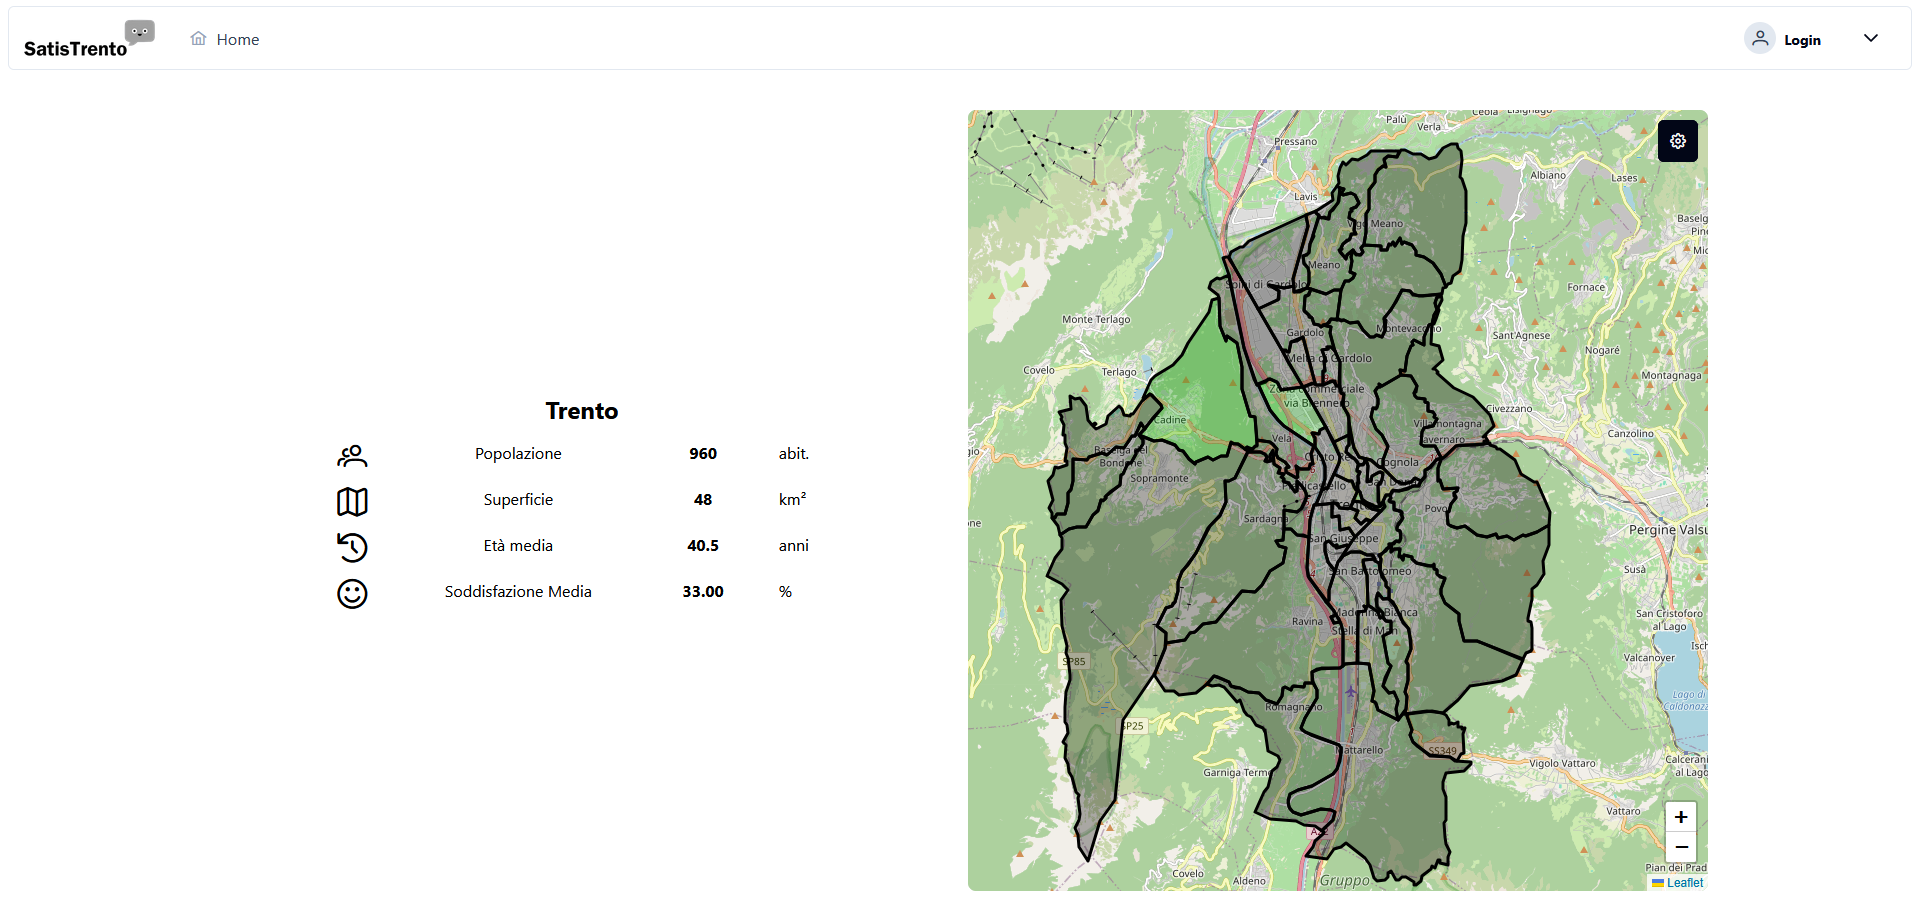
\includegraphics[width=0.8\textwidth]{frontend/home.png}
        \caption{\textit{Home Page} per utenti non loggati}
        \label{fig:frontend-home}
    \end{figure}
    Nella Figura \Ref{fig:frontend-home} è possibile vedere la \textit{Home Page} della \textit{web-app}. Come da specifiche descritte nei documenti precedenti questa presenta: i dati generali relativi all'intero comune, la mappa interattiva, tematica sulla base della soddisfazione media e suddivisa per quartieri. Nell'angolo in alto a destra della mappa è presente un pulsante per aprire il menù delle impostazioni per passare da ``quartieri'' a ``circoscrizioni'' e viceversa. Inoltre, nell'angolo superiore destro della pagina è presente un pulsante per accedere alla pagina di \textit{login}.
    
    \subsubsection{Dettaglio menù impostazioni}
        \begin{figure}[H]
            \centering
            
\includegraphics[width=0.3\textwidth]{frontend/opzioni_quart_circ.png}
            \caption{Menù impostazioni}
            \label{fig:frontend-settings}
        \end{figure}
        Come precedentemente descritto, il menù delle impostazioni sopra raffigurato, chiudibile premendo la ``X'', permette di passare da una visualizzazione dei dati per quartieri ad una per circoscrizioni e viceversa. La figura sopra è relativa a tutte le tipologie di utenti ad eccezione degli utenti con ruolo ``analista''.
\newpage
    \subsubsection{Selezione di un ``quartiere''/``circoscrizione''}
        \begin{figure}[H]
            \centering
            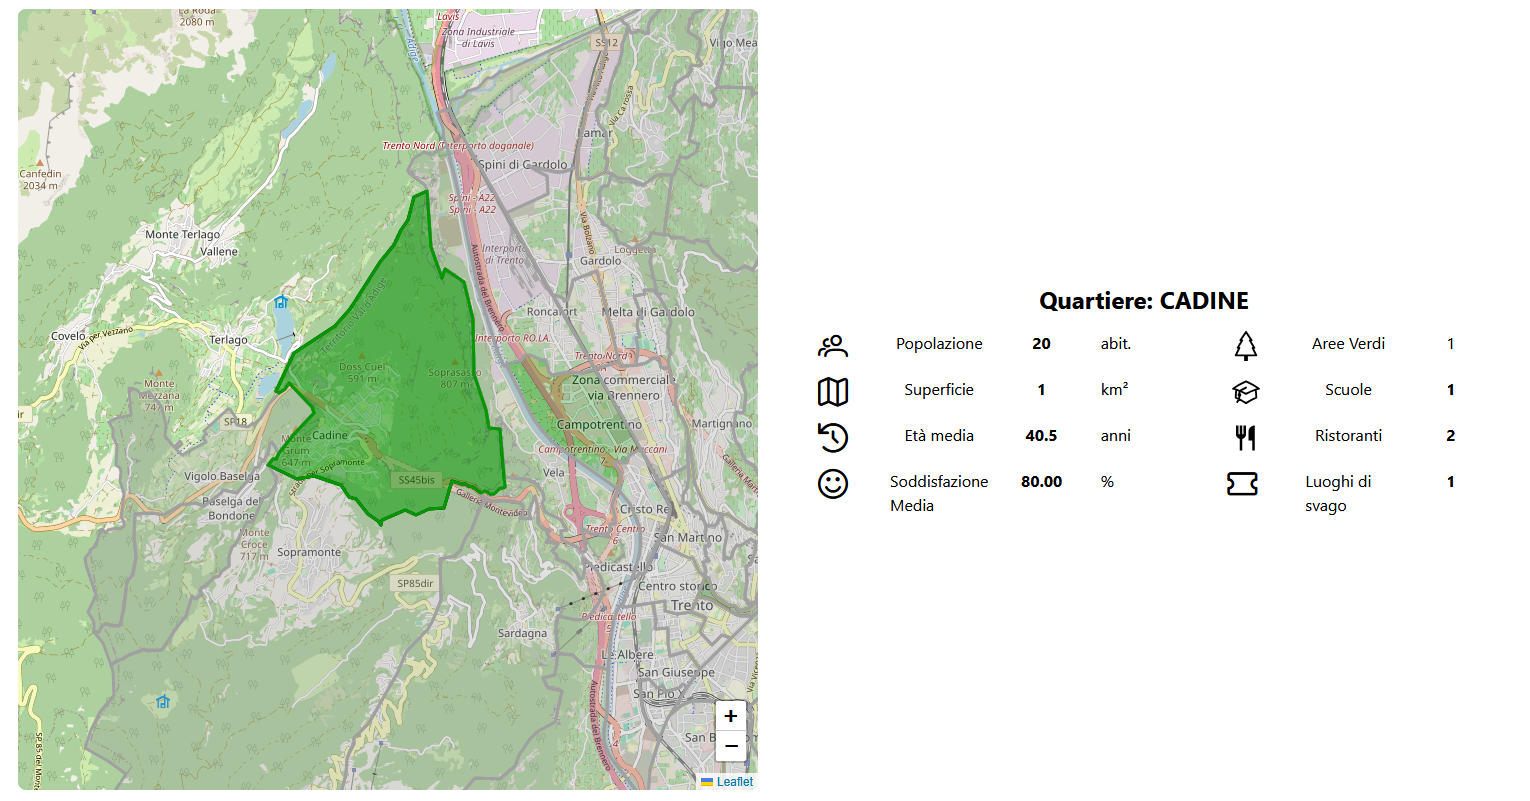
\includegraphics[width=0.8\textwidth]{frontend/quartiere_selezionato.png}
            \caption{Selezione di un ``quartiere''/``circoscrizione''}
            \label{fig:frontend-quartiere}
        \end{figure}
        Notiamo dalla Figura \Ref{fig:frontend-quartiere} come la selezione di un ``quartiere'' o ``circoscrizione'' avvenga tramite un click sulla mappa. Una volta selezionato un ``quartiere'' o ``circoscrizione'' verranno visualizzati degli ulteriori informazioni più specifiche riguardanti il ``quartiere'' o la ``circoscrizione'' selezionata. Inoltre il ``quartiere'' o la ``circoscrizione'' selezionata verrà evidenziata sulla mappa oscurano gli altri ``quartieri'' o le altre ``circoscrizioni'', inoltre la mappa avrà il suo centro sul centro del quartiere ed avrà uno zoom adeguato per visualizzare il ``quartiere'' o la ``circoscrizione'' selezionata nella sua interezza. Da questa schermata è possibile tornare alla visualizzazione generale ri-selezionando il ``quartiere'' o la ``circoscrizione'' selezionata oppure è possibile cambiare ``quartiere'' o ``circoscrizione'' selezionando un altro ``quartiere'' o ``circoscrizione'' dalla mappa.
\section{\textit{Login}}
    \begin{figure}[H]
        \centering
        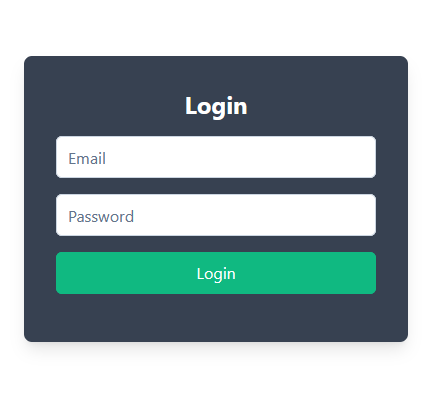
\includegraphics[width=0.4\textwidth]{frontend/dettaglio_login.png}
        \caption{Dettaglio pagina di \textit{login}}
        \label{fig:frontend-login}
    \end{figure}
    Nella Figura \Ref{fig:frontend-login} è possibile vedere il dettaglio della pagina di \textit{login}. Da questa pagina tutti gli utenti in possesso di credenziali valide possono accedere. \newpage
        \subsubsection{Messaggio di errore}
        \begin{figure}[H]
            \centering
            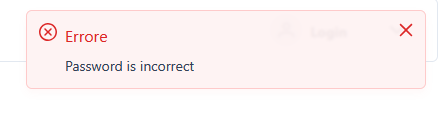
\includegraphics[width=0.4\textwidth]{frontend/dettaglio_errore_login.png}
            \caption{Messaggio di errore}
            \label{fig:frontend-login-error}
        \end{figure}
        Nella Figura \Ref{fig:frontend-login-error} è possibile vedere come si presenta il messaggio di errore in caso di credenziali errate. Questo viene visualizzato per $5$ secondi in caso di credenziali errate o altro errore.\newline
        Si noti come il presente ``formato'' di \textit{feedback} per i messaggi di errori sia stato implementato per tutte le pagine della \textit{web-app} in caso di un qualsiasi errore, viene difatti mostrato il titolo dell'errore con l'azione che non è stata possibile effettuare ed una descrizione più dettagliata del perché non è stato possibile effettuare l'azione richiesta.
        \subsubsection{Messaggio di login effettuato}
        \begin{figure}[H]
            \centering
            
\includegraphics[width=0.4\textwidth]{frontend/dettaglio_messaggio_login.png}
            \caption{Messaggio di login effettuato}
            \label{fig:frontend-login-success}
        \end{figure}
        Nella Figura \Ref{fig:frontend-login-success} è possibile vedere come si presenta il messaggio di login effettuato con successo. Questo viene visualizzato per $3$ secondi in caso di login effettuato con successo.\newline
        Si noti come il presente ``formato'' di \textit{feedback} sia stato implementato per tutte le pagine della \textit{web-app} in caso di un qualsiasi errore, viene difatti mostrato la scritta ``successo'', o altra equivalente, ed una breve descrizione di cosa è stato effettuato con successo.
\section{Funzionalità Analista}
    Nella seguente sezione verranno illustrate le funzionalità disponibili per gli utenti con ruolo ``analista''. Questi utenti hanno accesso a funzionalità specifiche per la loro mansione e non disponibili agli altri utenti.
    \begin{figure}[H]
        \centering
        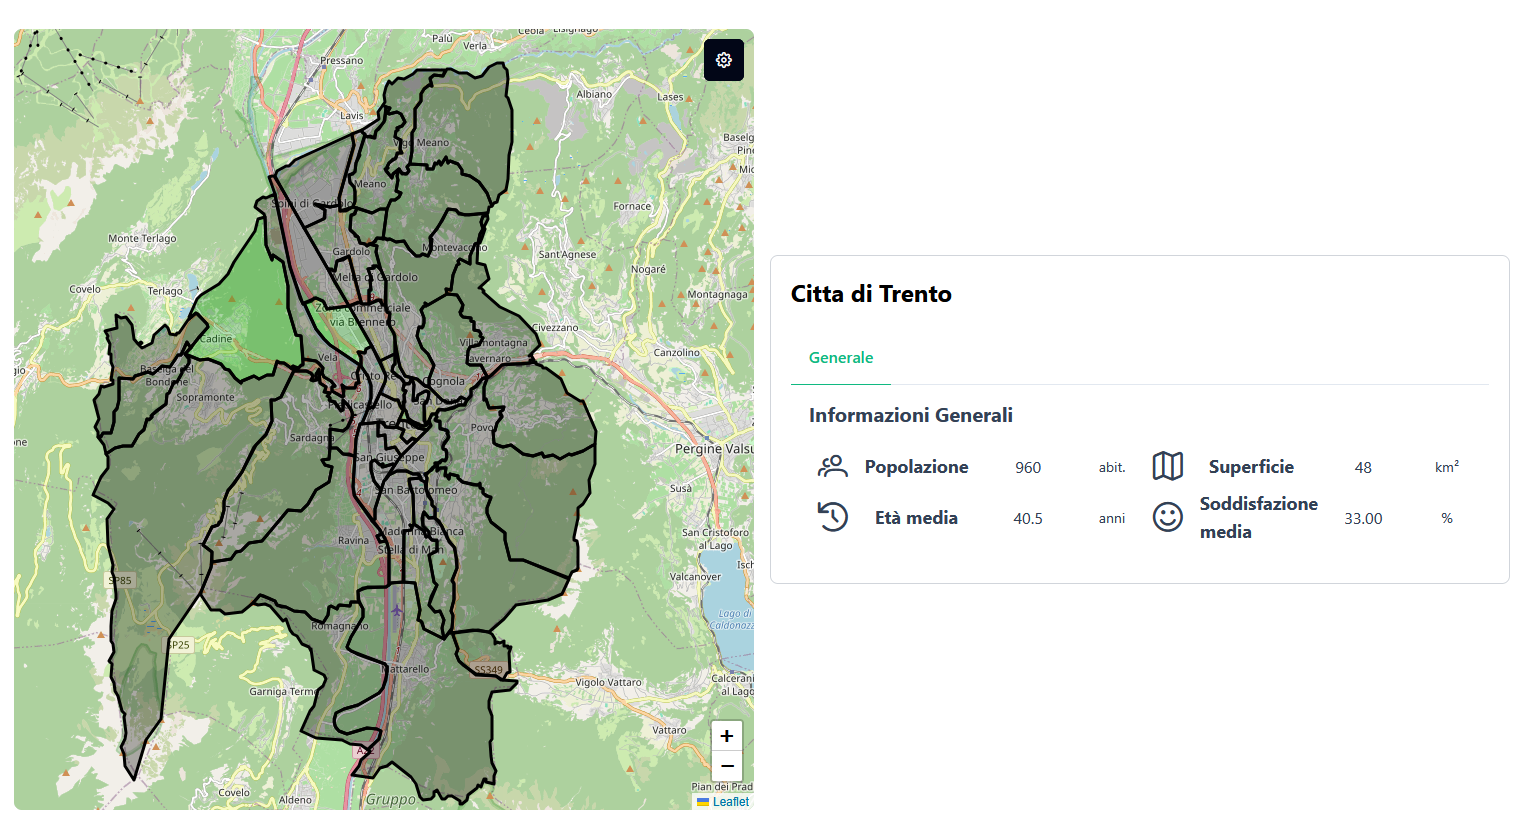
\includegraphics[width=0.8\textwidth]{frontend/home_analista.png}
        \caption{\textit{Home Page} per utenti con ruolo ``analista''}
        \label{fig:frontend-analista}
    \end{figure}
    Possiamo notare dalla Figura \Ref{fig:frontend-analista} come l'interfaccia grafica si sia differenziata rispetto alla Figura \Ref{fig:frontend-home}. Possiamo notare come le informazioni generali del comune siano comunque visibili ma sono raggruppate, non cambia molto infatti dalla \textit{homepage} delle altre tipologie di utenti. 
    \subsubsection{Selezione di un ``quartiere''/``circoscrizione'' - analista}
        \begin{figure}[H]
            \centering
            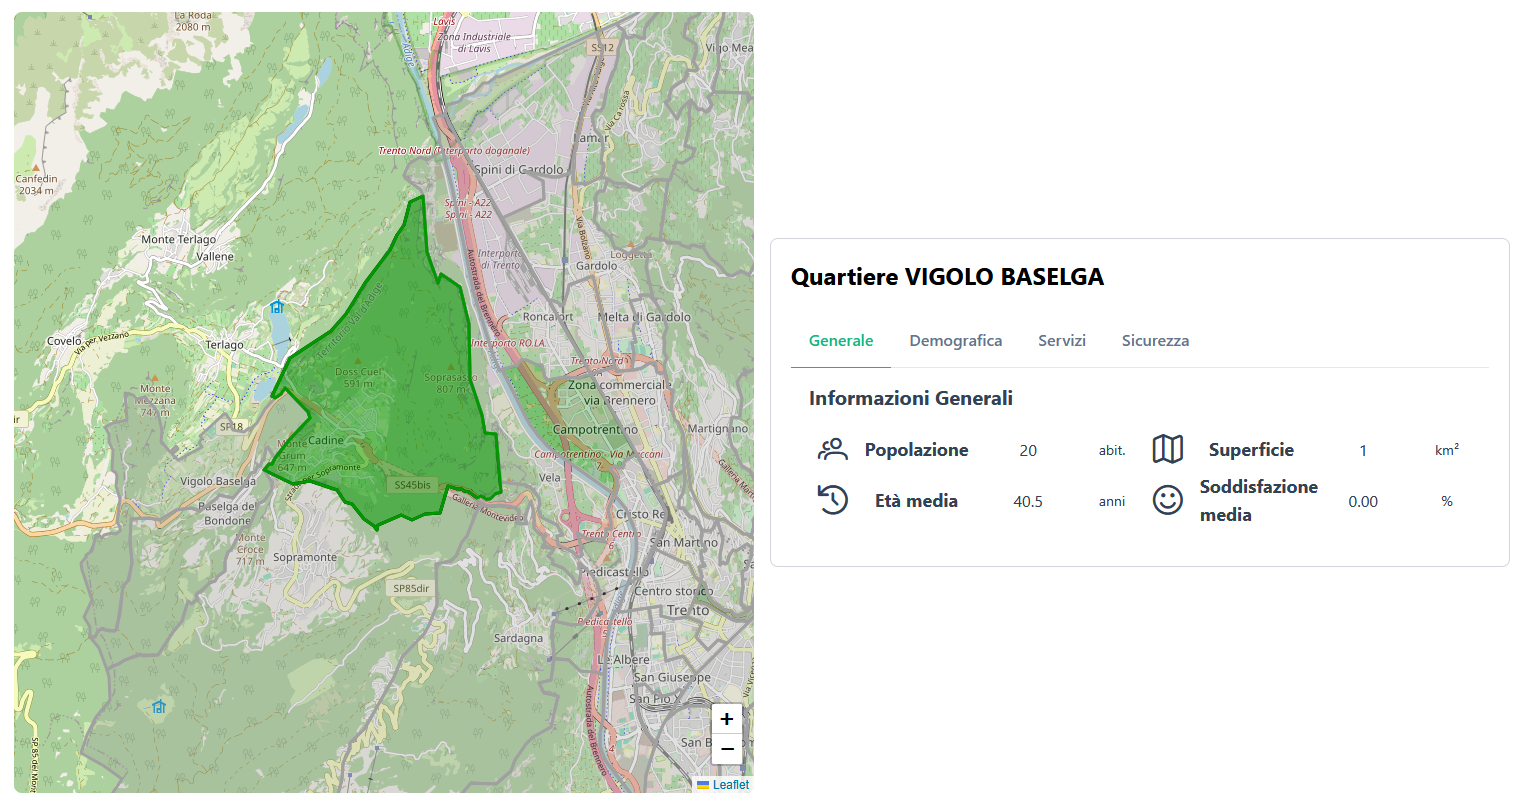
\includegraphics[width=0.8\textwidth]{frontend/alaisi_selezionato.png}
            \caption{Selezione di un ``quartiere''/``circoscrizione'' per utenti con ruolo ``analista''}
            \label{fig:frontend-analista-quartiere}
        \end{figure}
        Notiamo dalla Figura \Ref{fig:frontend-analista-quartiere} come la selezione di un ``quartiere'' o ``circoscrizione'' avvenga tramite un click sulla mappa come nel caso degli altri utenti. Una volta selezionato un ``quartiere'' o ``circoscrizione'' verranno visualizzati oltre alle informazioni generali del ``quartiere'' o della ``circoscrizione'' anche altri indicatori accessibili tramite le diverse pagine del menù posizionato sulla destra della mappa.\newline
        Si possa notare come questa visualizzazione sia una estensione della visualizzazione per gli altri utenti, dunque tutte le funzionalità e le azioni che il sistema compie alla selezione/deselezione sono le stesse.
    \subsubsection{Dettaglio menù impostazioni}
        \begin{figure}[H]
            \centering
            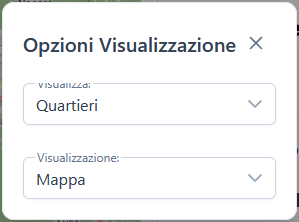
\includegraphics[width=0.3\textwidth]{frontend/opzioni_analista.png}
            \caption{Menù impostazioni per utenti con ruolo ``analista''}
            \label{fig:frontend-settings-analista}
        \end{figure}
        Il menù delle impostazioni per gli utenti con ruolo ``analista'' estende le funzionalità del menù per tutti gli altri utenti della figura \Ref{fig:frontend-settings}. In particolare, oltre alla possibilità di passare da una visualizzazione dei dati per quartieri ad una per circoscrizioni e viceversa, è possibile passare dalla visualizzazione di questi da una visualizzazione in ``mappa'' ad una in ``tabella''. Questo permette agli utenti con ruolo ``analista'' di avere una visione più dettagliata dei dati.
    \subsubsection{Visualizzazione dati in ``tabella''}
        \begin{figure}[H]
            \centering
            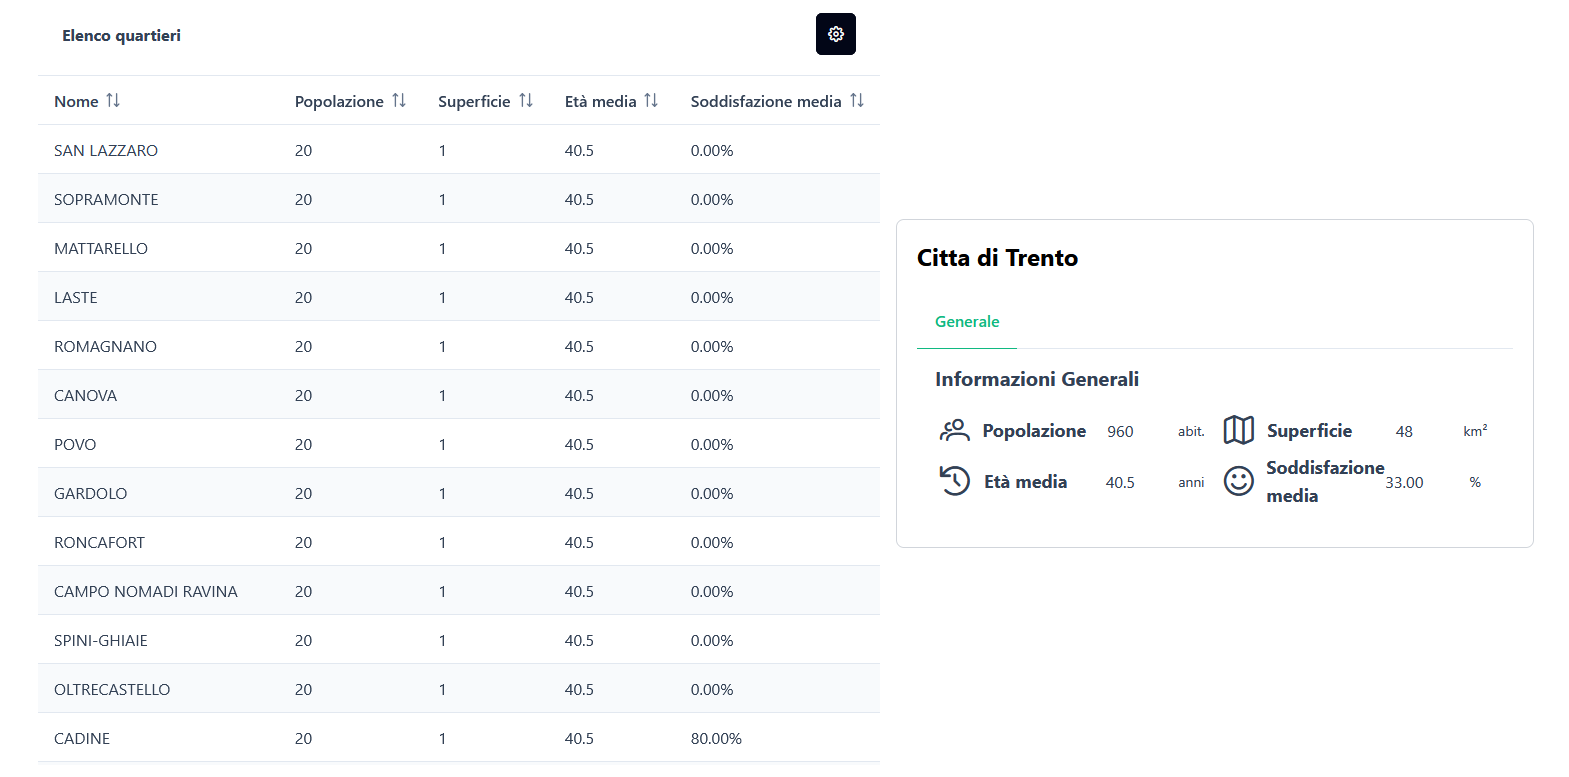
\includegraphics[width=0.8\textwidth]{frontend/home_analista_tabella.png}
            \caption{Visualizzazione dati in ``tabella''}
            \label{fig:frontend-analista-tabella}
        \end{figure}
        Nella Figura \Ref{fig:frontend-analista-tabella} è possibile vedere la visualizzazione dei dati in ``tabella'' per gli utenti con ruolo ``analista''. Questa visualizzazione permette di avere una visione, ordinabile per le colonne presenti, dei dati relativi ai ``quartieri'' o alle ``circoscrizioni''. Da questa visualizzazione è possibile selezionare un ``quartiere'' o una ``circoscrizione'' premendo sulla riga corrispondente. 
    \subsubsection{``Quartiere''/``circoscrizione'' selezionata in visualizzazione tabella}
        \begin{figure}[H]
            \centering
            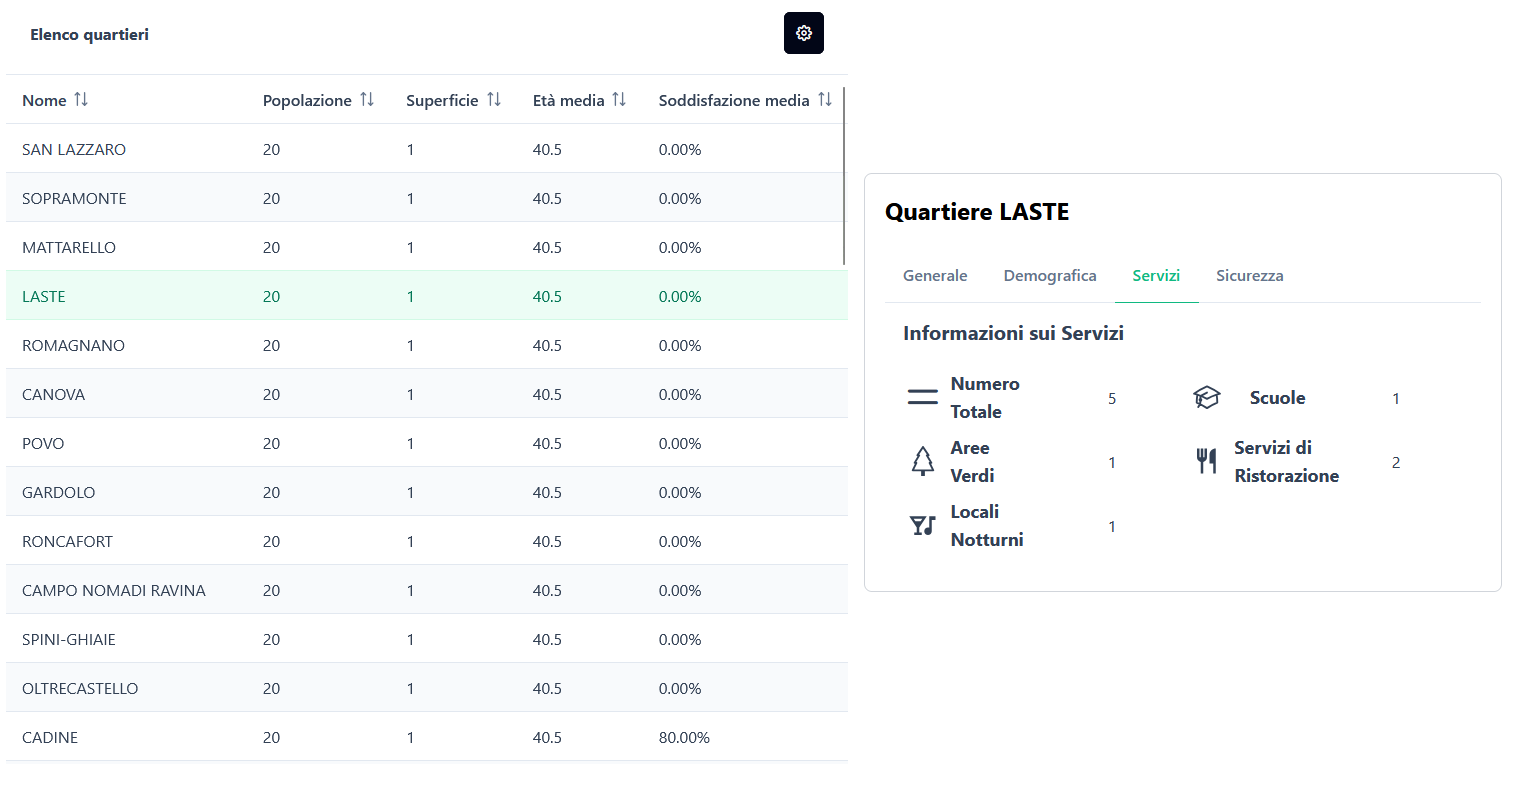
\includegraphics[width=0.8\textwidth]{frontend/alaisi_selezionato_tabella.png}
            \caption{``Quartiere''/``circoscrizione'' selezionata in visualizzazione tabella}
            \label{fig:frontend-analista-tabella-selezionato}
        \end{figure}
        La figura \Ref{fig:frontend-analista-tabella-selezionato} mostra come si presenta la visualizzazione di un ``quartiere'' o una ``circoscrizione'' selezionata in visualizzazione tabella. Questa situazione è una unione della selezione nel caso della figura \Ref{fig:frontend-analista-quartiere} e della visualizzazione in tabella della figura \Ref{fig:frontend-analista-tabella}. Da questa visualizzazione è possibile tornare alla visualizzazione dei dati della città selezionando il ``quartiere'' o la ``circoscrizione'' selezionata oppure è possibile cambiare ``quartiere'' o ``circoscrizione'' selezionando un altro ``quartiere'' o ``circoscrizione'' dalla tabella, in questo caso la riga selezionata verrà evidenziata ed i dati relativi al ``quartiere'' o alla ``circoscrizione'' selezionata verranno visualizzati.
\section{Funzionalità Sondaggista}
    Si illustrano in questa sezione tutte le funzionalità disponibili per gli utenti con ruolo ``sondaggista''. Questi utenti hanno accesso a funzionalità specifiche per effettuare sondaggi, gestirli ed inviarli per l'approvazione. La visualizzazione della \textit{Home Page} per gli utenti con ruolo ``sondaggista'' è la stessa di quella degli altri utenti, come mostrato nella figura \Ref{fig:frontend-home}.
    \subsubsection{Gestione sondaggi}
        \begin{figure}[H]
            \centering
            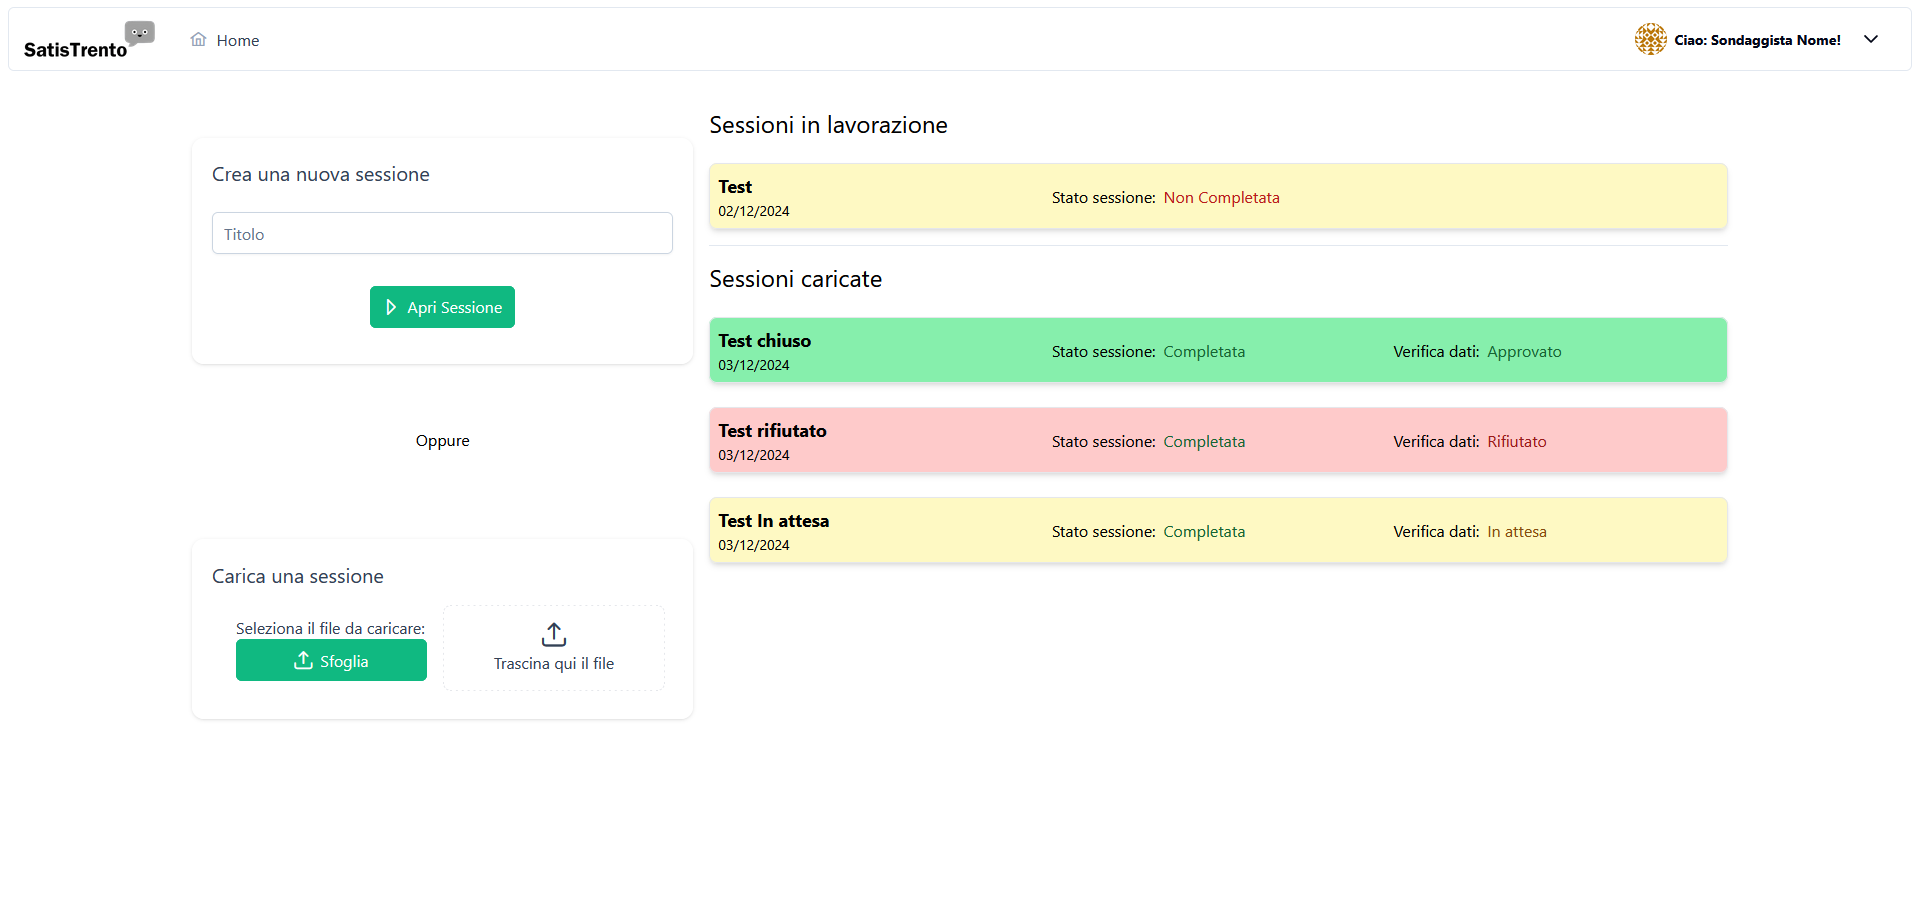
\includegraphics[width=0.8\textwidth]{frontend/sondaggista_home.png}
            \caption{Pagina di gestione dei sondaggi}
            \label{fig:frontend-sondaggista}
        \end{figure}
        Nella figura \Ref{fig:frontend-sondaggista} è possibile vedere la pagina di gestione dei sondaggi per gli utenti con ruolo ``sondaggista''. Da questa pagina è possibile iniziare un nuovo sondaggio tramite il modulo con pulsante nella parte superiore-sinistra della pagina, caricare un sondaggio da un file \textit{.csv} tramite il pulsante nella parte inferiore-sinistra della pagina\footnote{Funzionalità non implementata} ed infine è possibile vedere l'elenco dei sondaggi in corso e quelli inviati per l'approvazione. Possiamo distinguere come lo stato del sondaggio, oltre che riportato nella riga stessa del sondaggio, sia rappresentato da un colore diverso per ogni stato. In particolare, il colore verde indica che il sondaggio è stato approvato, il colore giallo indica che il sondaggio è in attesa di approvazione o se presente sotto la voce ``Sessioni in lavorazione'' indica che il sondaggio è in corso, il colore rosso indica che il sondaggio è stato rifiutato.\newline
        I sondaggi ``in lavorazione'' ovvero quelli in corso, sono visualizzati in una sezione separata rispetto a quelli inviati per l'approvazione. Questo in quanto i sondaggi in corso sono quelli che possono essere modificati e completati, mentre quelli inviati per l'approvazione non possono più essere modificati dai sondaggisti. È presente per questi sondaggi un pulsante per visualizzare e riprendere il sondaggio, in modo da poterlo completare e inviare per l'approvazione.
    \newpage
    \subsubsection{Pagina gestione sondaggio}
        \begin{figure}[H]
            \centering
            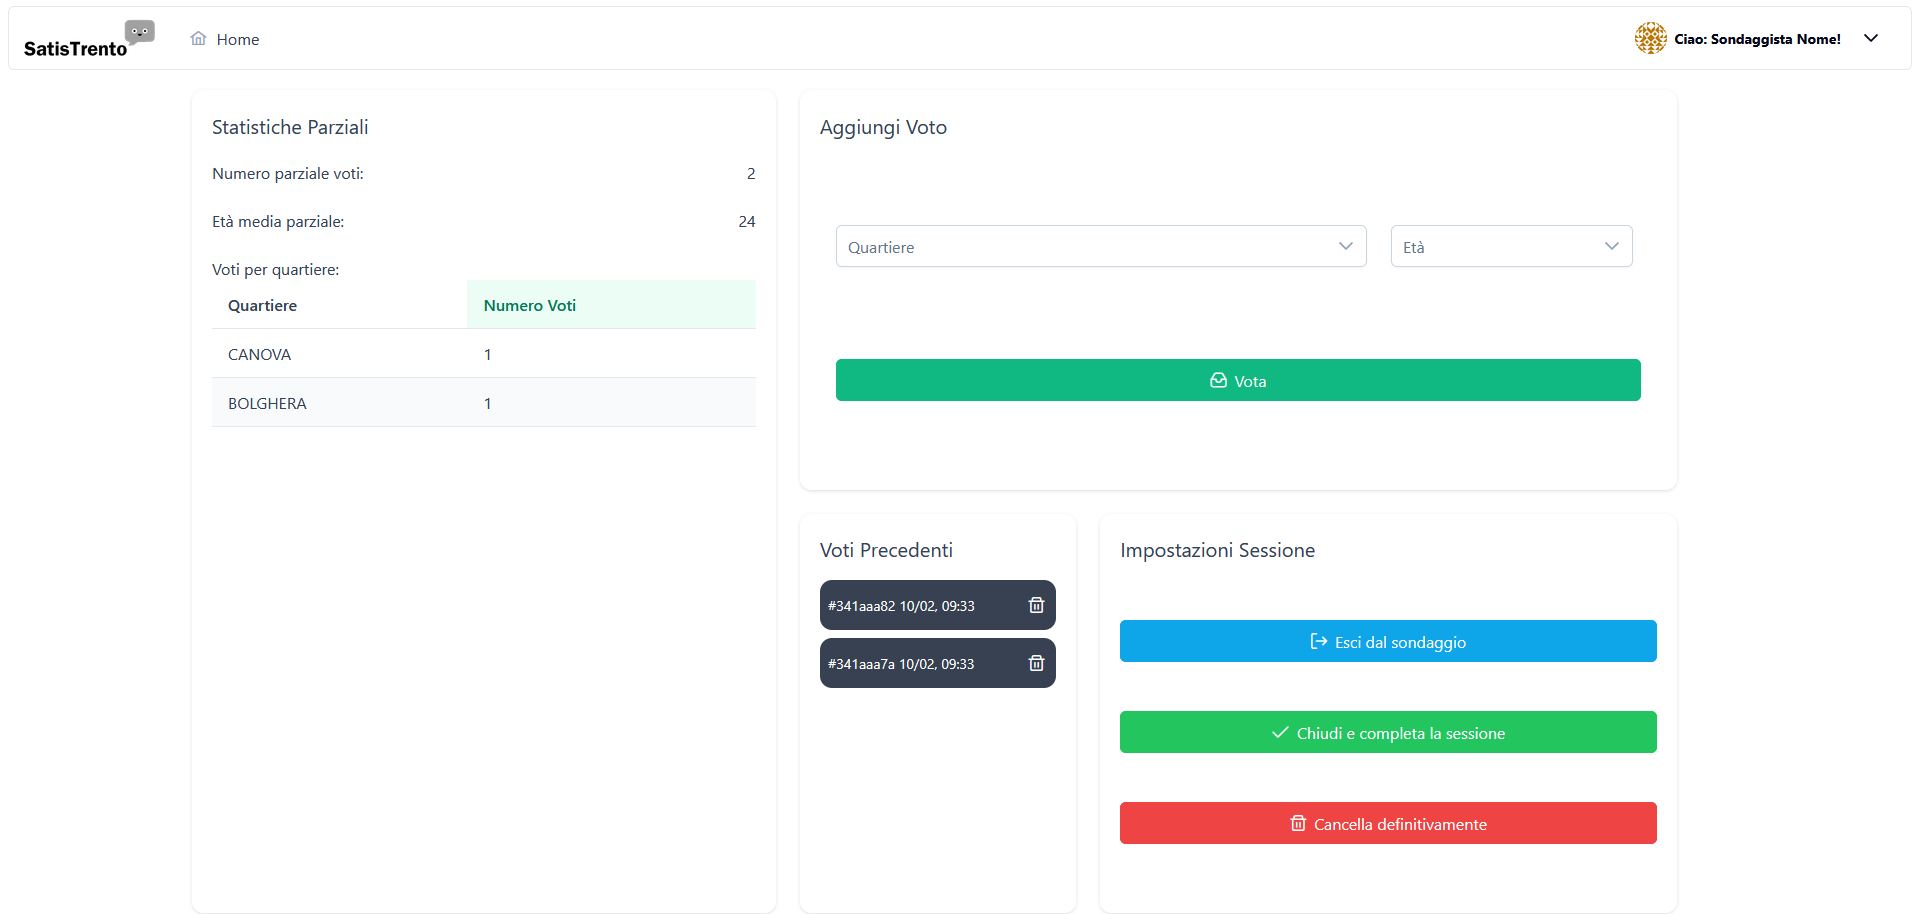
\includegraphics[width=0.8\textwidth]{frontend/gestione_sondaggio.png}
            \caption{Pagina di gestione di un sondaggio}
            \label{fig:frontend-gestione-sondaggio}
        \end{figure}
        La pagina mostrata dalla figura \Ref{fig:frontend-gestione-sondaggio} si può dividere in quattro aree, sulla parte sinistra è possibile individuare le ``Statistiche parziali'' ovvero: il numero di voti raccolti fino ad ora, l'età media dei votanti, ed una tabella contenente il numero di voti per ogni quartiere di provenienza dei votanti. Nel riquadro che occupa la parte superiore centrale e superiore destra è presente il pre-modulo per l'inserimento di un voto all'interno del sondaggio, questi si compongono di due selettori del tipo ``menù a discesa'', uno per il quartiere di appartenenza (obbligatorio impostarne il valore) ed uno per l'età del votante (opzionale). Nella parte centrale inferiore è presente l'elenco dei voti già inseriti, per motivi di \textit{privacy} si è scelto di non mostrare il voto, ma solo un identificativo ed l'orario di inserimento, questo in quanto la possibilità di eliminare un voto è fornita solo per la correzione di errori. Infine nella parte inferiore destra sono presenti i controlli per uscire dal sondaggio e tornare all'elenco dei sondaggi, per inviare il sondaggio per l'approvazione e per eliminare il sondaggio.
    \subsubsection{Dettaglio invio sondaggio/eliminazione sondaggio}
        \begin{figure}[H]
            \centering
            
\includegraphics[width=0.4\textwidth]{frontend/dettaglio_conferma_chiusura.png}
            \caption{Dettaglio invio sondaggio}
            \label{fig:frontend-conferma-chiusura}
        \end{figure}
        Nella figura \Ref{fig:frontend-conferma-chiusura} è possibile vedere il dettaglio della finestra di conferma per l'invio del sondaggio per l'approvazione. Questa finestra di conferma è presente anche per l'eliminazione del sondaggio, col pulsante di eliminazione colorato di rosso ed altri testi, ma con la stessa struttura. Questa finestra di conferma è presente per evitare eliminazioni accidentali di sondaggi o invii accidentali per l'approvazione.
    \subsubsection{Processo di voto}
        \begin{figure}[H]
            \centering
            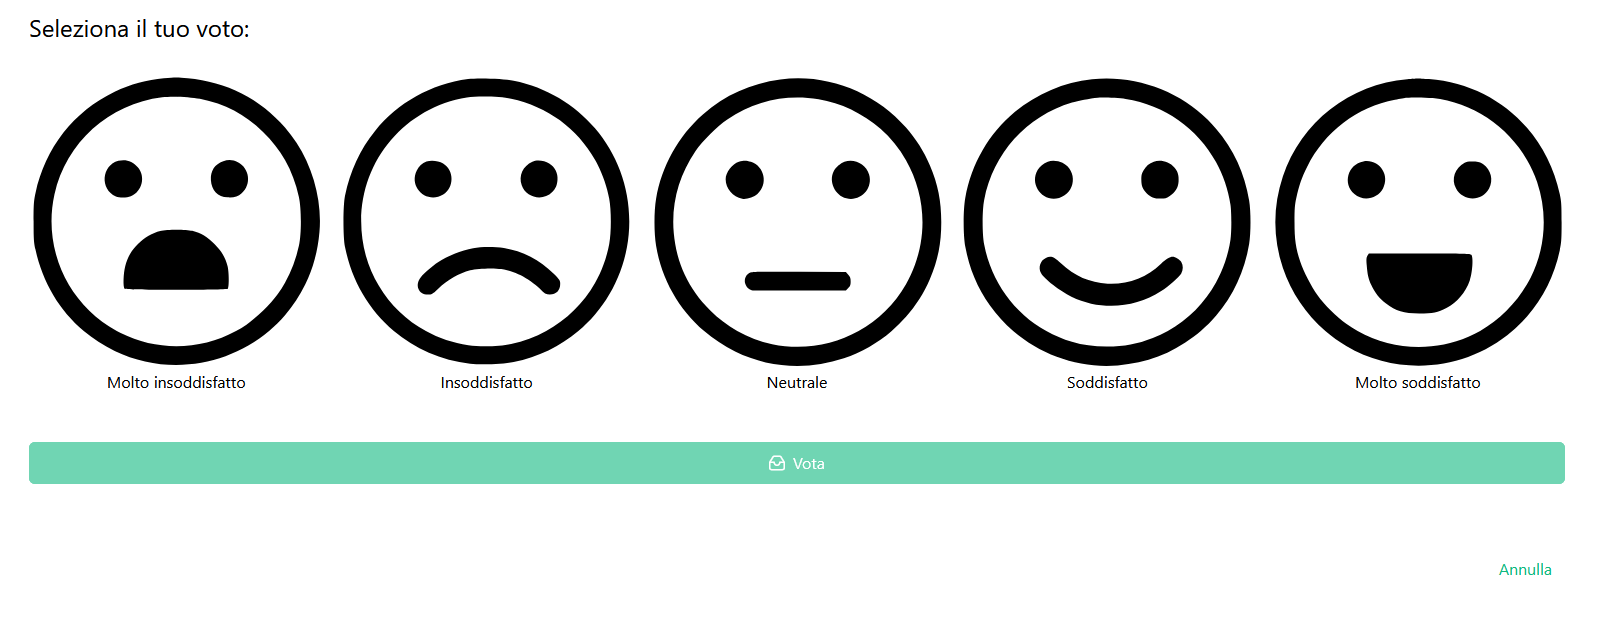
\includegraphics[width=0.8\textwidth]{frontend/dettaglio_voto.png}
            \caption{Dettaglio pagina di voto}
            \label{fig:frontend-voto}
        \end{figure}
        Dalla presente figura \Ref{fig:frontend-voto} si può notare come si presenta al votante l'interfaccia di voto dopo che il sondaggista ha compilato ``quartiere'' ed opzionalmente ``età'' del votante e premuto il tasto ``vota''. 
        \begin{figure}[H]
            \centering
            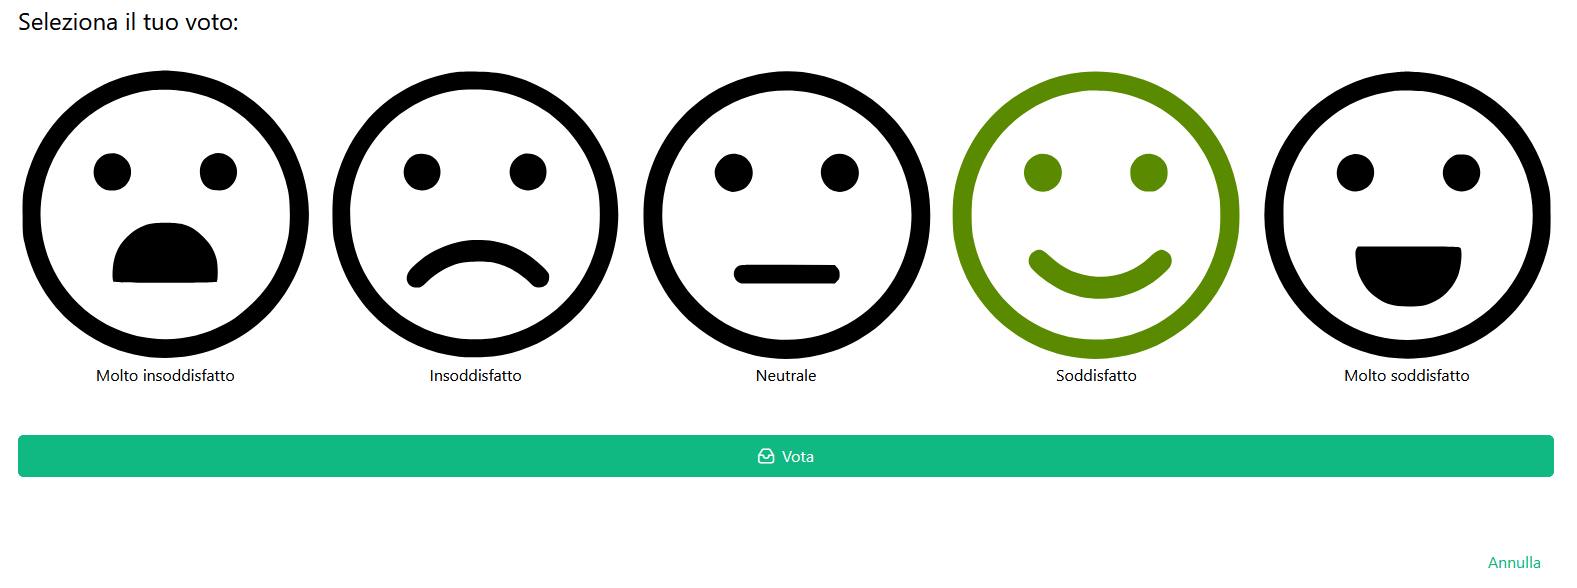
\includegraphics[width=0.8\textwidth]{frontend/dettaglio_voto_selezionato.png}
            \caption{Dettaglio pagina di voto con voto selezionato}
            \label{fig:frontend-voto-selezionato}
        \end{figure}
        Dalla figura \Ref{fig:frontend-voto-selezionato} si può notare come si presenta al votante l'interfaccia di voto dopo che il votante ha selezionato il voto. Il voto è selezionabile tramite un click su uno dei pulsanti con il voto desiderato. Una volta selezionato il voto il pulsante selezionato verrà evidenziato con un colore diverso dagli altri pulsanti. Una volta selezionato il voto è possibile confermare il voto premendo il pulsante ``vota'' oppure se sono stati commessi degli errori nella pre-compilazione del voto è possibile annullare il voto premendo il pulsante ``annulla''.
        \begin{figure}[H]
            \centering
            
\includegraphics[width=0.8\textwidth]{frontend/dettaglio_post_voto.png}
            \caption{Dettaglio pagina di voto post-voto}
            \label{fig:frontend-voto-post}
        \end{figure}
        Una volta che l'utente ha confermato il voto, verrà visualizzata la pagina di conferma del voto come mostrato nella figura \Ref{fig:frontend-voto-post}. A questo punto il dispositivo dovrebbe essere restituito al sondaggista il quale tornerà tramite il pulsante ``chiudi'' alla pagina di gestione del sondaggio.